%%%%%%%%%%%%%%%%%%%%%%%%%%%%%%%%%%%%%%%%%%%%%%
%                insertmeeting
% 1) Title (something creative & funny?)
% 2) Date (MM/DD/YYYY)
% 3) Location (ex. Hagerty High School)
% 4) People/Committees Present 
% 5) Picture 
% 6) Start Time & Stop Time (ex. 12:30AM to 4:30PM)
%%%%%%%%%%%%%%%%%%%%%%%%%%%%%%%%%%%%%%%%%%%%%%
\insertmeeting 
	{Imaginative Implementations} 
	{01/11/22} 
	{Hagerty High School}
	{Annika, Anouska, Clayton, Falon, James, Jensen, Nathan, Ritam, Rose, Samantha, Lilly}
	{Images/RobotPics/robot.jpg}
	{2:30 - 4:30}
	
\hhscommittee{Software}
\noindent\hfil\rule{\textwidth}{.4pt}\hfil
\subsubsection*{Goals}
\begin{itemize}
    \item Begin to implement our derived tricycle kinematic equations into an extendible Kotlin class.   

\end{itemize} 

\noindent\hfil\rule{\textwidth}{.4pt}\hfil

\subsubsection*{Accomplishments}
After verifying that our tricycle kinematic equations were correct, we wanted to begin implementing it into our code. This was a monumental task, as it involved modifying existing localization systems while ensuring that they can still work with the pre-existing TRC event systems and Road Runner. But to simplify that task, we broke it down into smaller portions. Our first goal was to create classes similar to "TankDrive" and "TankKinematics" in the Road Runner library that would be able to hold the methods and data we will need for our tricycle drive. We started by using a template from the sample Tank Drive Kinematics provided by Road Runner. We took the localization calculations and inserted them where the tank kinematic equations were. This new file, "TricycleKinematics.kt" allowed us to continue localization the robot using our uncommon wheel encoder tracking. We would later use these functions in a class titled "TricycleDrive.kt" that represented the drivebase to use in Road Runner. It contained modified methods to update() the drive position using the new tricycle kinematics equations. Next, we have to test these methods in conjunction with Road Runner to find any errors. 
 

\begin{figure}[htp]
\centering
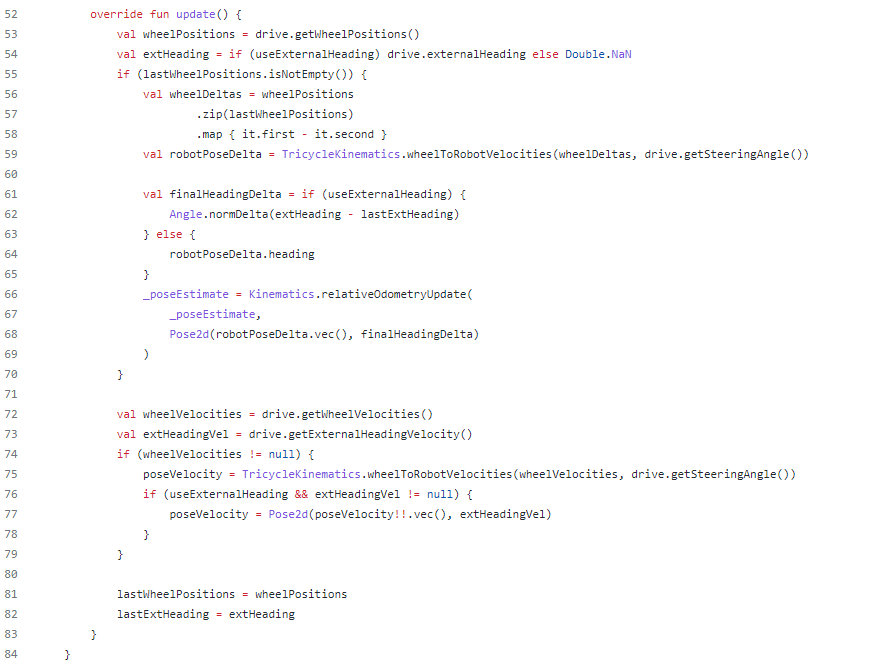
\includegraphics[width=0.95\textwidth, angle=0]{Meetings/January/01-11-22/1.13.22 tricyledrive.kt - James Hu.PNG}
\caption{Our update method, created based on samples provided by Road Runner}
\label{fig:011122_1}
\end{figure}

\begin{figure}[htp]
\centering
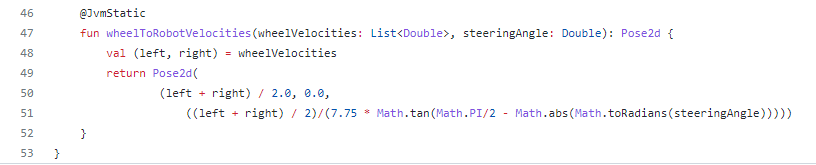
\includegraphics[width=0.95\textwidth, angle=0]{Meetings/January/01-11-22/1.13.22 tricyledrivekinematics.kt - James Hu.PNG}
\caption{Implementing the new kinematic equations into our code}
\label{fig:011122_2}
\end{figure}


\whatsnext{
\begin{itemize}
    \item Ensure that TricycleRRDrive works well with Road Runner before we begin to implement TRC event systems. 
\end{itemize} 
}

